\documentclass[10pt,a4paper]{article}
\usepackage[margin=15mm]{geometry}
\usepackage{amsmath,booktabs,pdfpages,hyperref}
\pagestyle{plain}
\begin{document}
\begin{center}\Large Au+Au 3.85 GeV: $\Lambda$--$^4$He CF in four $m_T$ slices\\
\large Centrality 0--10\%, KFParticle\end{center}
\noindent CF: 20 MeV/c; display 0-0.3 GeV/c; normalization 0.30-0.40 GeV/c.

\medskip
\noindent The fixed boundaries are specified in YAML and coincide with stored
0.05 GeV/$c^2$ edges. They are not moved to equalize counts.
Only the configured $m_T$ range is included; tails outside it are excluded.
Excluded signal pairs for $0\leq k^*<0.3$ GeV/$c$: below range SE=0, ME=0; above range SE=237, ME=7842.

The same slices are used for both methods, SE, ME and sidebands.

\begin{center}\small\begin{tabular}{rrrrrr}\toprule
Slice & $m_T$ [GeV/$c^2$] & SE (0--0.3) & ME (0--0.3) & SE norm & ME norm\\\midrule
1 & 2.40–2.60 & 12175 & 436803 & 20366 & 759268 \\
2 & 2.60–2.80 & 31746 & 1141675 & 39621 & 1454986 \\
3 & 2.80–3.00 & 12532 & 453695 & 13637 & 495936 \\
4 & 3.00–3.20 & 2224 & 80082 & 2392 & 85425 \\
\bottomrule\end{tabular}\end{center}

\noindent\textbf{Method 5 is an approximation, not an $m_T$-resolved mass fit.}
The available histograms have no joint $(k^*,m_T,M_\Lambda)$ distribution.
The same $m_T$-integrated, centrality-0--10\% $P_{SE}(k^*)$ and $P_{ME}(k^*)$
are applied to all four slices. Purity grid: 50 MeV/$c$;
five-bin sliding window: 250 MeV/$c$ in the interior.
Each original 5 MeV/$c$ count is weighted before summing to 20 MeV/$c$.

\medskip
\noindent Constant purity: $P=0.96721065$ (the same inclusive proxy as before),
with $C_{corr}=[C_{sig}-(1-P)C_{SB}]/P$. Sidebands and normalization
are evaluated separately in each $m_T$ slice.

\medskip
\noindent Approximate errors include shared purity reuse and normalization.
Covariances between mass-fit backgrounds and observed counts, distinct overlapping
fits, $m_T$ counts and inclusive purity, and reused event/mixed pairs are not available.
Constant-$P$ errors are conditional on fixed $P$.
Sparse/zero-SE bins do not have Poisson confidence intervals.
The smallest SE signal bins contain only a few pairs despite the large slice totals.
Exact candidate mass gates and whole mass-bin fit integrals differ slightly.

\medskip
\noindent 2021 P24iy only; 26,956/26,994 subjobs in this partial merge.
The input ROOT and all production cuts are unchanged.
Full provenance, statistics and caveats are in the adjacent README and JSON files.
\medskip\noindent\textbf{Masked points (not zero):} mT 3.00-3.20, constant\_purity, k* 0.00-0.02. Zero ME denominators / invalid normalization are not filled.
\clearpage
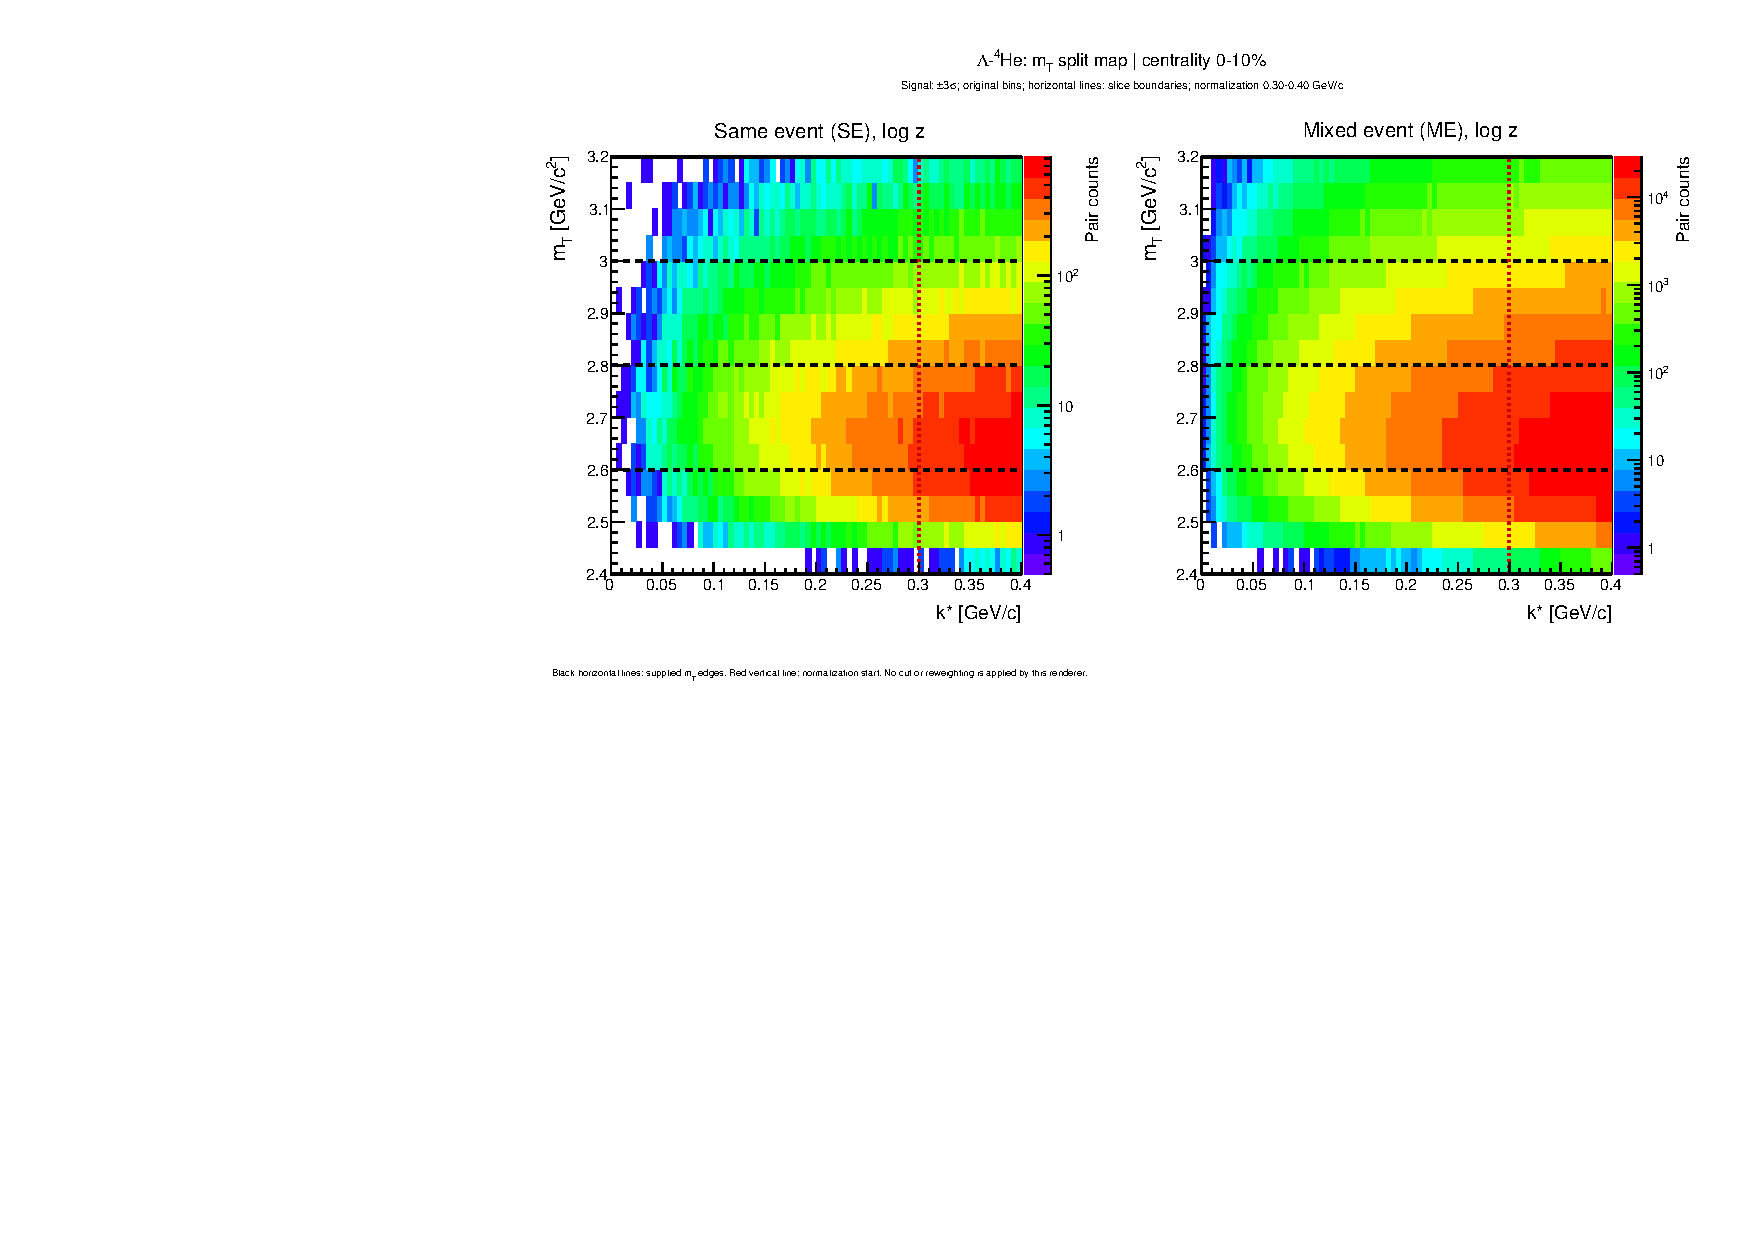
\includepdf[pages=-]{mt_distribution.pdf}
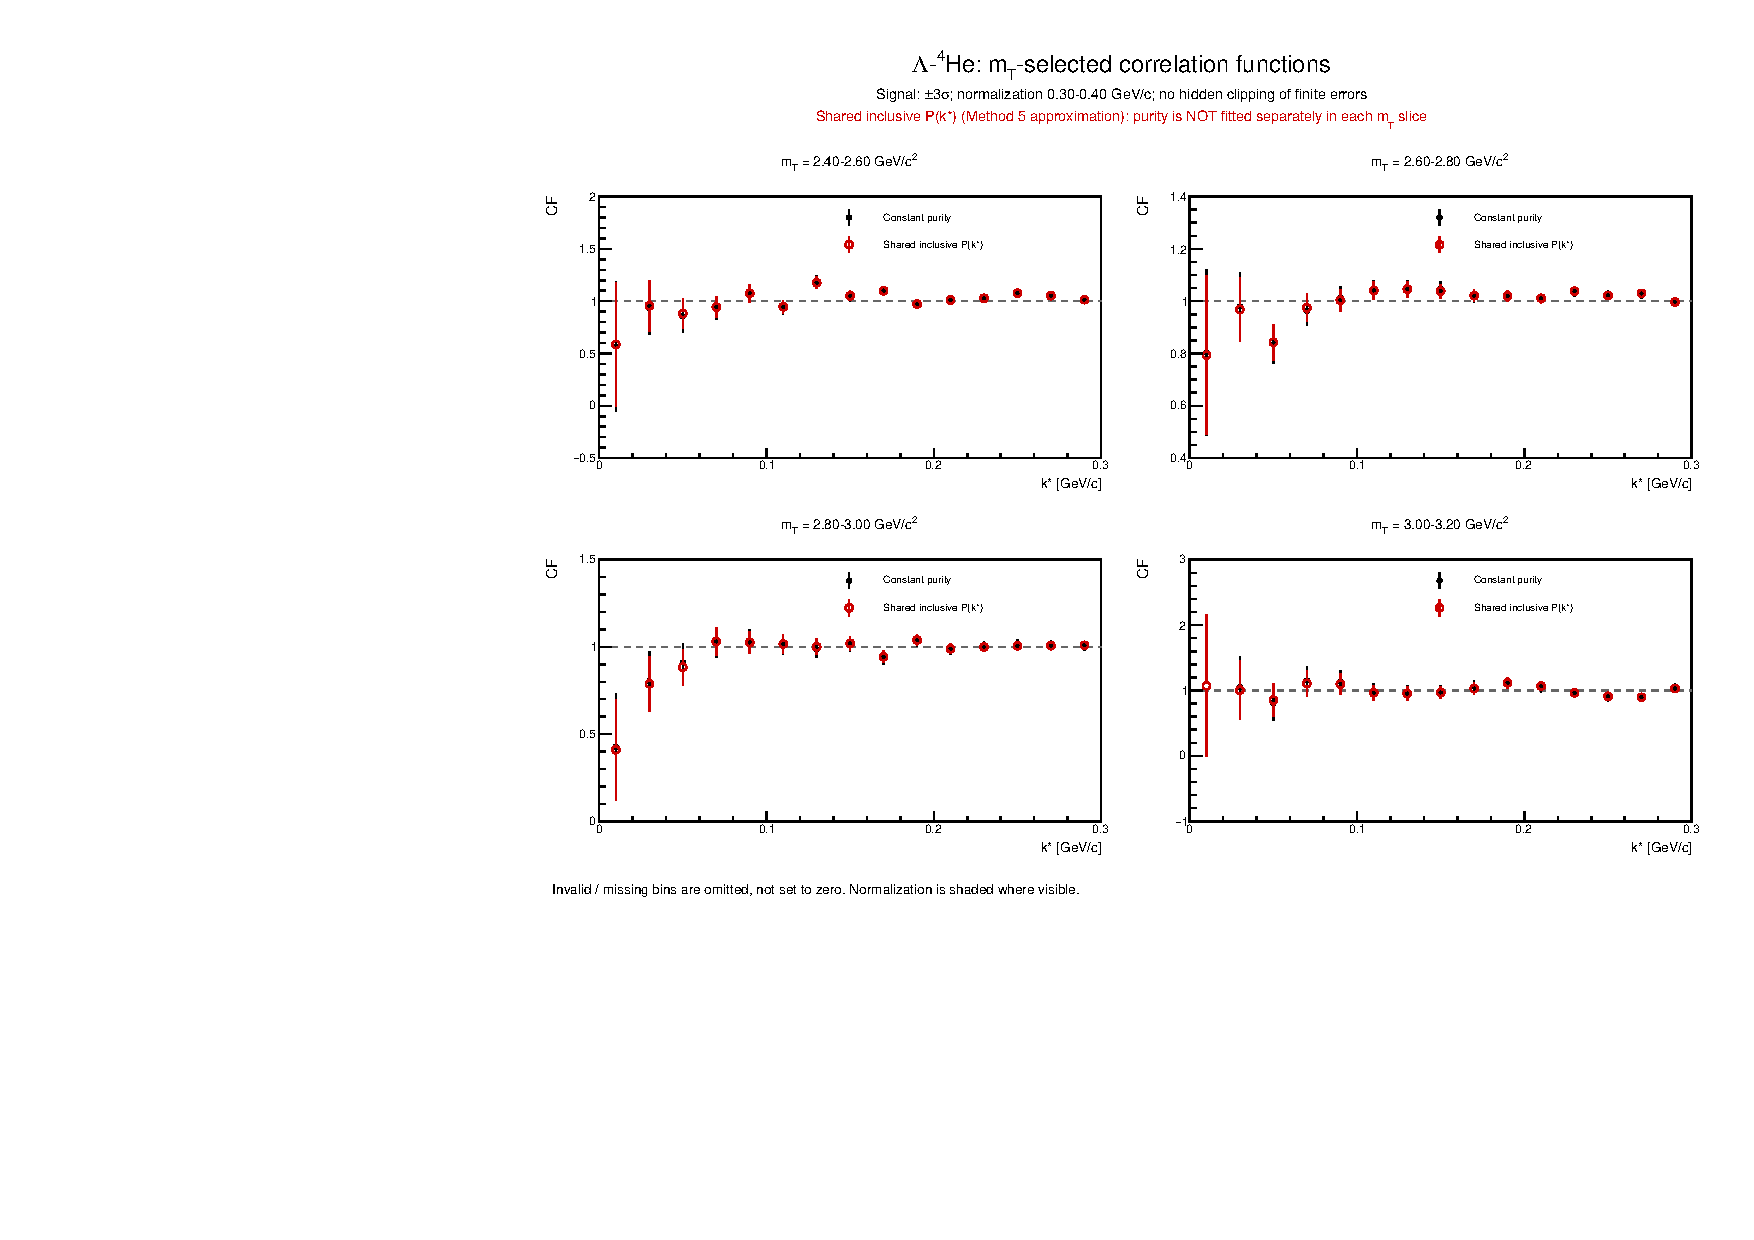
\includepdf[pages=-]{mt_cf_comparison.pdf}
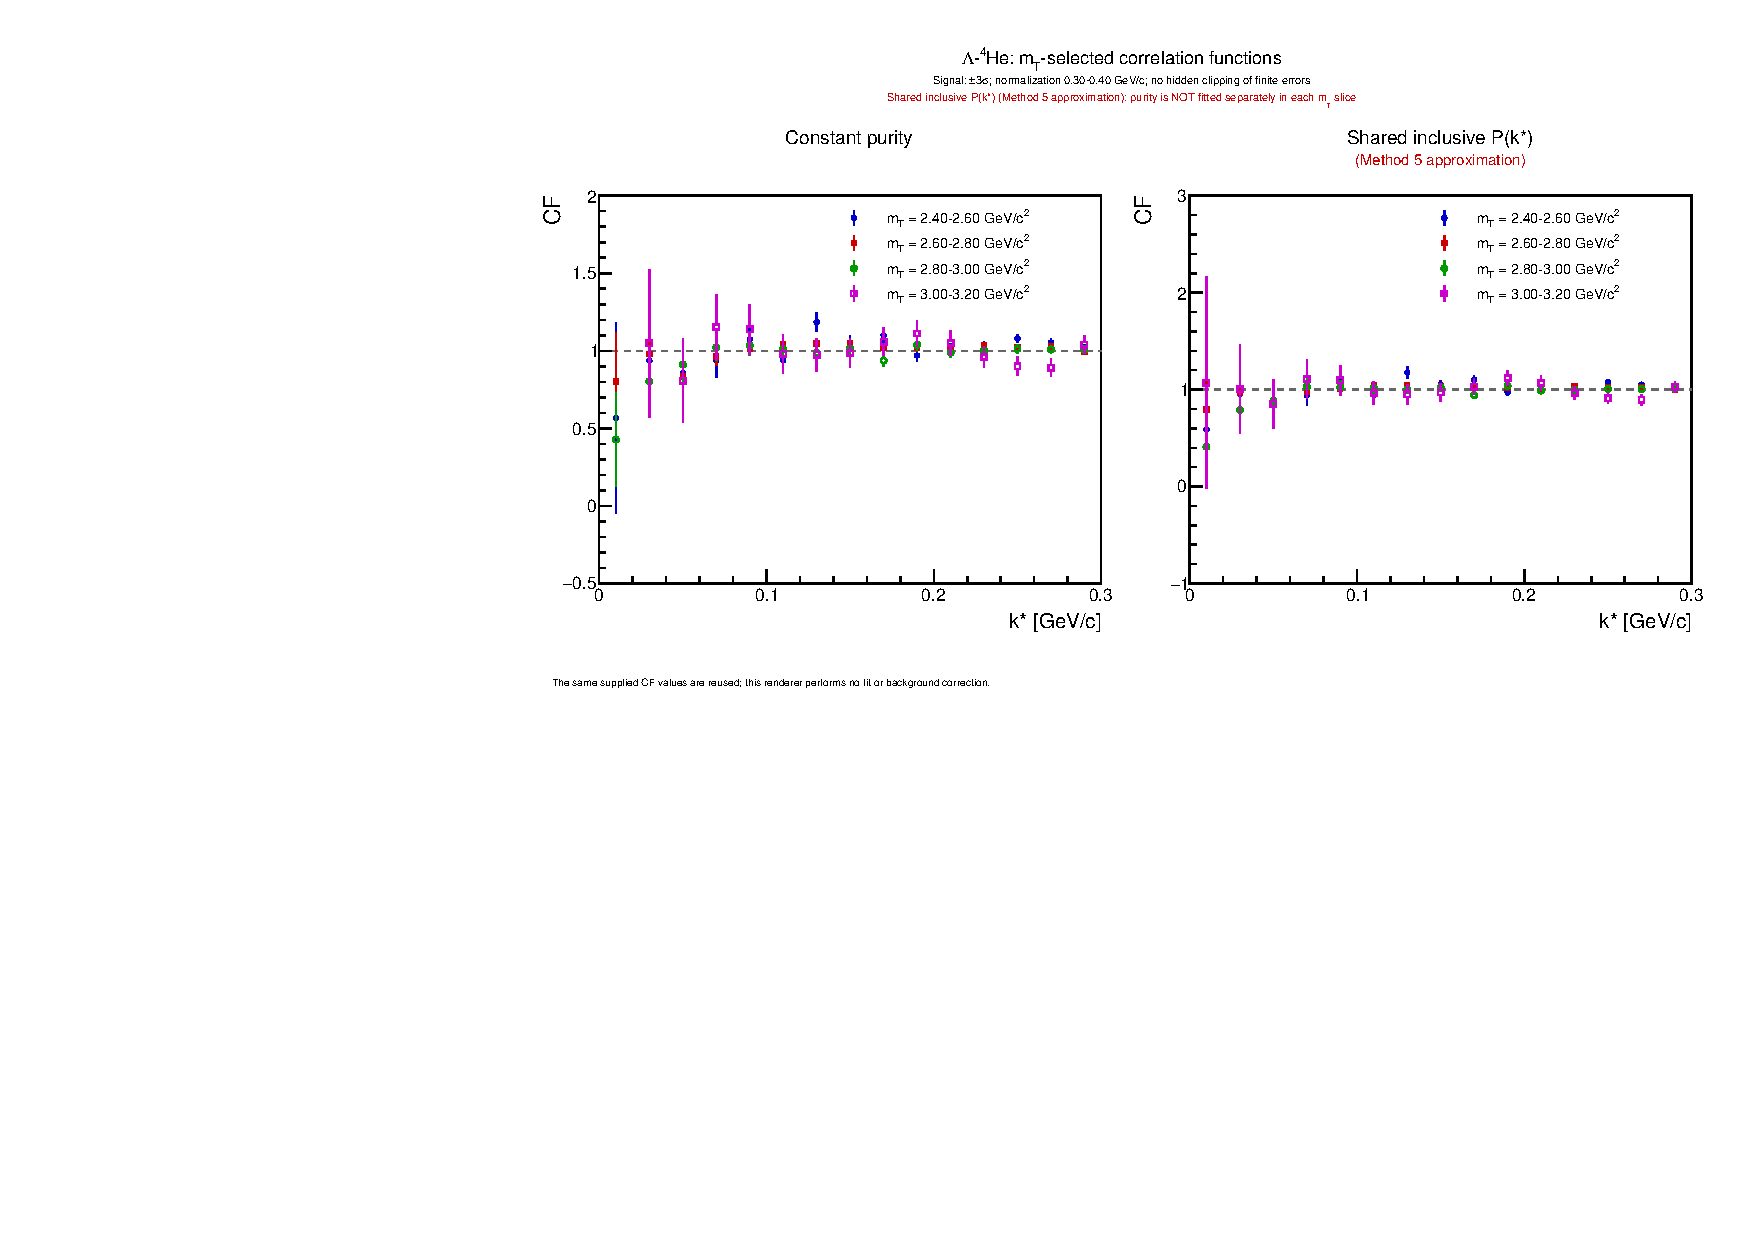
\includepdf[pages=-]{mt_cf_overlays.pdf}
\end{document}
